\documentclass[12pt]{article}

\textwidth 16cm \textheight 23cm \evensidemargin 0cm
\oddsidemargin 0cm \topmargin -2cm
\parindent 0pt
\parskip \medskipamount

\usepackage[utf8]{inputenc}
\usepackage[dutch]{babel}
\usepackage{amssymb}
\usepackage{amsmath}
\usepackage{amsthm}
\usepackage{hyperref}
\usepackage{enumerate}
\usepackage{subfig}
\usepackage{wrapfig}
\usepackage{minibox}
\usepackage{ifthen}
\usepackage{dot2texi}
\usepackage{multicol}
\usepackage{graphicx}
\usepackage{cancel}
%\usepackage{fix-cm}
\usepackage{setspace}
\usepackage{mdframed}
\usepackage{mathtools}
%\usepackage{lipsum}

\usepackage{exsol}
\renewcommand{\exercisename}{}
\renewcommand{\solutionname}{}

\usepackage{fancyhdr}
\pagestyle{fancy}

\usepackage{color}
\newcommand{\todo}[1]{\textcolor{red}{\##1\#}}
\newcommand{\question}[1]{\textcolor{blue}{\##1\#}}

\newcommand{\vraag}[2]{\begin{itemize}\item {\it #1} \vspace*{#2}\end{itemize}}

\newcommand{\degree}{\ensuremath{^\circ}}
\def\LRA{\Leftrightarrow\mkern40mu}

\newcommand\ggd{\qopname\relax o{\mathrm{ggd}}}
\newcommand\kgv{\qopname\relax o{\mathrm{kgv}}}

\newcounter{menucount}\newcounter{curitem}% Counters
\newcommand{\menuitem}{\texttt}% Menu item formatting
\newcommand{\menusep}{\ensuremath{\rightarrow}}% Menu separator
\newcommand{\menuend}{\relax}% Menu end
\newcommand{\menulist}[1]{% \menulist{<menu list>}
  \setcounter{menucount}{0}\setcounter{curitem}{0}% Reset menucount & curitem
  \renewcommand*{\do}[1]{\stepcounter{menucount}}%
  \menulistparser{#1}% Count menu items
  \renewcommand*{\do}[1]{\menuitem{##1}\stepcounter{curitem}\ifnumless{\value{curitem}}{\value{menucount}}{\menusep}{\menuend}}%
  \menulistparser{#1}% Process list
}
\DeclareListParser{\menulistparser}{:}% List separator is ':'

%\graphicspath{{../figuren/}}

\newcommand{\dotrule}[1]{%
   \parbox[t]{#1}{\vspace*{3pt}\dotfill}}
   
\newcommand{\dotFill}{\vspace*{6pt}\dotfill}

\newcommand{\dotlines}[1]{   
\foreach \n in {1,...,#1}{

\vspace*{0.1cm}
\dotfill
\vspace*{0.1cm}
}}

\newcommand{\ruitjes}[1]{

\hskip-2.6cm
\begin{tikzpicture}[scale=1.075,x=1.0cm,y=1.0cm]
\draw [help lines, solid, gray, very thin, step=0.5cm] (0,-#1+0.1cm) grid (21.6,-0.1);
\end{tikzpicture}
\vspace*{-1cm}
}

\newcommand{\ruitjesxy}[2]{
\begin{tikzpicture}[scale=1.01,line cap=round,line join=round,>=triangle 45,x=1.0cm,y=1.0cm]
\draw [color=cqcqcq,dash pattern=on 1pt off 1pt, xstep=0.4.5cm, ystep=0.4.5cm] (0,-#2) grid (#1,0);
\end{tikzpicture}
}

\newcommand{\zrmbox}{\framebox{\phantom{EXE}}\phantom{X}}
\newcommand{\zrm}[1]{\framebox{#1}}

% arule* answerrules
\def\arulefill{\xrfill[-0.5ex]{0.1pt}[lightgray]}
\newcommand{\arules}[1]{
\color{lightgray}
\vspace*{0.10cm}
\foreach \n in {1,...,#1}{
  \vspace*{0.70cm}
  \hrule height 0.1pt\hfill
}\color{black}}
\newcommand{\arule}[1]{
\color{lightgray}{\raisebox{-0.1cm}{\rule[-0.05cm]{#1}{0.1pt}}}\color{black}
}

% environment oefening:
% houdt een teller bij die de oefeningen nummert
% probeert ook de oefening op één pagina te houden
\newcounter{noefening}
\setcounter{noefening}{0}
\newenvironment{oefening}
{
  \stepcounter{noefening}
  \begin{minipage}{\textwidth}
  \vspace*{8pt}{\large\bf Oefening \arabic{noefening}}
}{%
  \end{minipage}
}

% environment voorbeeld:
% houdt een teller bij die de voorbeelden nummert
% nummering herbegint bij elke subsectie
% probeert het voorbeeld op één pagina te houden
\newcounter{nvb}[subsection]
%\@addtoreset{nvb}{subsubsection}
\setcounter{nvb}{0}
\newenvironment{voorbeeld}
{
  \stepcounter{nvb}
  \begin{minipage}{\textwidth}
  \vspace*{4pt}
  \textit{Voorbeeld \arabic{nvb}}\\[5pt]
}{%
  \end{minipage}
}

% environment voorbeeld*:
% probeert het voorbeeld op één pagina te houden
\newenvironment{voorbeeld*}
{
  \begin{minipage}{\textwidth}
  \vspace*{4pt}
  \textit{Voorbeeld}
}{%
  \end{minipage}
}

\newenvironment{onthoud}
{
\begin{mdframed}[nobreak=true,frametitle={Te onthouden}]
}{%
\end{mdframed}
}

\newcommand{\vglproef}[2]{LL= #1\;${=\joinrel=}$\; RL= #2}

\newcommand{\getallenas}[3][1]{
\definecolor{cqcqcq}{rgb}{0.65,0.65,0.65}
\begin{tikzpicture}[scale=#1,line cap=round,line join=round,>=triangle 45,x=1.0cm,y=1.0cm]
\draw [color=cqcqcq,dash pattern=on 1pt off 1pt, xstep=1.0cm,ystep=1.0cm] (#2,-0.2) grid (#3,0.2);
\draw[->,color=black] (#2,0) -- (#3,0);
\draw[shift={(0,0)},color=black] (0pt,2pt) -- (0pt,-2pt) node[below] {\footnotesize $0$};
\draw[shift={(1,0)},color=black] (0pt,2pt) -- (0pt,-2pt) node[below] {\footnotesize $1$};
\draw[color=black] (#3.25,0.07) node [anchor=south west] {$\mathbb{R}$};
\end{tikzpicture}
}

\newcommand{\opdracht}{{\bf Opdracht }}

% geef tabular iets meer ruimte
\setlength{\tabcolsep}{15pt}
\renewcommand{\arraystretch}{1.5}

% geef align iets meer ruimte:
\addtolength{\jot}{0.5em}

\newtheorem{definition}{Definitie}
\newtheorem{eigenschap}{Eigenschap}

\newcommand{\visgraad}[1]{\begin{tabular}{p{0.5cm}|p{#1}}&\\\hline\\\end{tabular}}

\newcommand{\assenstelsel}[5][1]{
\definecolor{cqcqcq}{rgb}{0.65,0.65,0.65}
\begin{tikzpicture}[scale=#1,line cap=round,line join=round,>=triangle 45,x=1.0cm,y=1.0cm]
\draw [color=cqcqcq,dash pattern=on 1pt off 1pt, xstep=1.0cm,ystep=1.0cm] (#2,#4) grid (#3,#5);
\draw[->,color=black] (#2,0) -- (#3,0);
\draw[shift={(1,0)},color=black] (0pt,2pt) -- (0pt,-2pt) node[below] {\footnotesize $1$};
\draw[color=black] (#3.25,0.07) node [anchor=south west] { x};
\draw[->,color=black] (0,#4) -- (0,#5);
\draw[shift={(0,1)},color=black] (2pt,0pt) -- (-2pt,0pt) node[left] {\footnotesize $1$};
\draw[color=black] (0.09,#5.25) node [anchor=west] { y};
\draw[color=black] (0pt,-10pt) node[right] {\footnotesize $0$};
\end{tikzpicture}
}

\newcommand{\ConfigureExSol}{
\renewcommand{\exercisename}{A.C.O.}
\renewcommand{\solutionname}{A.C.O.}
\newcounter{exercise2}[section]
\setcounter{exercise2}{0}
\renewcommand{\theexercise}{%
    \arabic{exercise2}%
}
\renewenvironment{exsol@exercise}[0]
{%
\refstepcounter{exercise2}
  \begin{minipage}[t]{\textwidth}%
    \ifthenelse{\boolean{exsol@exerciseaslist}}
               {\begin{list}%
                   {%
                   }%
                   {%
                     \setlength{\topsep}{0pt}%
                     \setlength{\leftmargin}{1em}%
                     \setlength{\rightmargin}{1em}%
                     \setlength{\listparindent}{0em}%
                     \setlength{\itemindent}{0em}%
                     \setlength{\parsep}{\parskip}}%
                 \item[\hspace*{\leftmargin}\textit{\exercisename{}
                                                    \theexercise:}]
               }%
               {
                 \textbf{\exercisename{} \theexercise:}~
               }
}
{%
  \ifthenelse{\boolean{exsol@exerciseaslist}}
             {\end{list}}{}
  \end{minipage}
  \vspace{1ex}\par
}
}

\onehalfspacing
%singlespacing
%doublespacing



\usepackage{tikz}
\usetikzlibrary{calc,arrows}
\newcommand{\tikzmark}[1]{\tikz[overlay,remember picture] \node (#1) {};}

%%%%%%%%%%%%%%%%%%%%%%%%%%%%%%%%%%%%%%%%%%
% Volgende wijzigingen werden aangebracht tov de originele bis-basis
% * 

%%%%%%%%%%%%%%%%%%%%%%%%%%%%%%%%%%%%%%%%%%
% Volgende opmerkingen heb ik nog
% * 

\lhead{}
\rhead{BIS-Basis -- Les 7}

\begin{document}

\ConfigureExSol

\setcounter{section}{6}
\section{Breuken}


\subsection{Begrippen}

$$\dfrac{\tikzmark{a}2}{\tikzmark{c}5}\qquad \begin{matrix}\tikzmark{b}\mbox{teller}\\\tikzmark{d}\mbox{noemer}\end{matrix} $$

\begin{tikzpicture}[overlay,remember picture,out=15,in=165,distance=0.5cm]
\draw[-stealth,shorten >=3pt,shorten <=10pt] (a.north) to (b.north);
\end{tikzpicture}
\begin{tikzpicture}[overlay,remember picture,out=345,in=195,distance=0.5cm]
\draw[-stealth,shorten >=0pt,shorten <=5pt] (c.east) to (d.west);
\end{tikzpicture}

Teller en noemer noemen we de {\bf termen} van de breuk.

\subsubsection{Wat is een breuk?}

We kunnen een breuk beschouwen als een aantal gelijke delen van een geheel.
De noemer duidt aan in hoeveel gelijke delen een geheel verdeeld is.
De teller zegt hoeveel gelijke delen er genomen worden.

\begin{voorbeeld}\\[0.5cm]
$\dfrac{2}{3}$\hspace*{1em}\raisebox{-1em}{
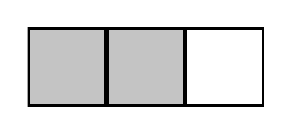
\begin{tikzpicture}[line cap=round,line join=round,>=triangle 45,x=1.0cm,y=1.0cm]
\clip(0,0) rectangle (3,1);
\draw [line width=1.6pt] (0,0) -- (1,0) -- (1,1) -- (0,1) -- cycle;
\fill [line width=1.6pt,fill=black,fill opacity=0.23] (0,0) -- (1,0) -- (1,1) -- (0,1) -- cycle;
\draw [line width=1.6pt] (1,0) -- (2,0) -- (2,1) -- (1,1) -- cycle;
\fill [line width=1.6pt,fill=black,fill opacity=0.23] (1,0) -- (2,0) -- (2,1) -- (1,1) -- cycle;
\draw [line width=1.6pt] (2,0) -- (3,0) -- (3,1) -- (2,1) -- cycle;
\end{tikzpicture}}
\end{voorbeeld}

\begin{voorbeeld}\\[0.5cm]
$\dfrac{1}{4}$\hspace*{1em}\raisebox{-1em}{
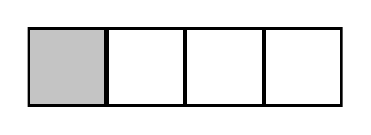
\begin{tikzpicture}[line cap=round,line join=round,>=triangle 45,x=1.0cm,y=1.0cm]
\clip(0,0) rectangle (4,1);
\draw [line width=1.6pt] (0,0) -- (1,0) -- (1,1) -- (0,1) -- cycle;
\fill [line width=1.6pt,fill=black,fill opacity=0.23] (0,0) -- (1,0) -- (1,1) -- (0,1) -- cycle;
\draw [line width=1.6pt] (1,0) -- (2,0) -- (2,1) -- (1,1) -- cycle;
\draw [line width=1.6pt] (2,0) -- (3,0) -- (3,1) -- (2,1) -- cycle;
\draw [line width=1.6pt] (3,0) -- (4,0) -- (4,1) -- (3,1) -- cycle;
\end{tikzpicture}}
of
\raisebox{-2em}{
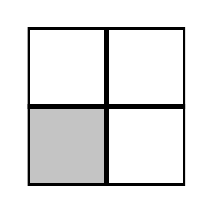
\begin{tikzpicture}[line cap=round,line join=round,>=triangle 45,x=1.0cm,y=1.0cm]
\clip(0,0) rectangle (2,2);
\draw [line width=1.6pt] (0,0) -- (1,0) -- (1,1) -- (0,1) -- cycle;
\fill [line width=1.6pt,fill=black,fill opacity=0.23] (0,0) -- (1,0) -- (1,1) -- (0,1) -- cycle;
\draw [line width=1.6pt] (1,0) -- (2,0) -- (2,1) -- (1,1) -- cycle;
\draw [line width=1.6pt] (1,1) -- (2,1) -- (2,2) -- (1,2) -- cycle;
\draw [line width=1.6pt] (0,1) -- (1,1) -- (1,2) -- (0,2) -- cycle;
\end{tikzpicture}}
\end{voorbeeld}

\begin{voorbeeld}\\[0.5cm]
$\dfrac{3}{2}$\hspace*{1em}\raisebox{-1em}{
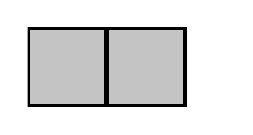
\begin{tikzpicture}[line cap=round,line join=round,>=triangle 45,x=1.0cm,y=1.0cm]
\clip(0,0) rectangle (2.5,1);
\draw [line width=1.6pt] (0,0) -- (1,0) -- (1,1) -- (0,1) -- cycle;
\fill [line width=1.6pt,fill=black,fill opacity=0.23] (0,0) -- (1,0) -- (1,1) -- (0,1) -- cycle;
\draw [line width=1.6pt] (1,0) -- (2,0) -- (2,1) -- (1,1) -- cycle;
\fill [line width=1.6pt,fill=black,fill opacity=0.23] (1,0) -- (2,0) -- (2,1) -- (1,1) -- cycle;
\end{tikzpicture}
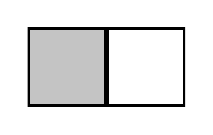
\begin{tikzpicture}[line cap=round,line join=round,>=triangle 45,x=1.0cm,y=1.0cm]
\clip(0,0) rectangle (2,1);
\draw [line width=1.6pt] (0,0) -- (1,0) -- (1,1) -- (0,1) -- cycle;
\fill [line width=1.6pt,fill=black,fill opacity=0.23] (0,0) -- (1,0) -- (1,1) -- (0,1) -- cycle;
\draw [line width=1.6pt] (1,0) -- (2,0) -- (2,1) -- (1,1) -- cycle;
\end{tikzpicture}}
\end{voorbeeld}

Een breuk kunnen we ook beschouwen als een andere schrijfwijze van een deling.
Als we $5 : 2$ uitrekenen bekomen we het geheel getal $2$ met rest $1$ of een decimaal getal $2.5$. In plaats van met decimalen te rekenen, kunnen we het resultaat ook schrijven in breukvorm.
$$5 : 2 = \dfrac{5}{2}$$

\begin{voorbeeld}
$$\dfrac{4}{7}=4:7$$
\end{voorbeeld}

\subsubsection*{Opmerkingen}
\begin{itemize}
  \item Schrijf de breukstreep steeds horizontaal.
  \item De noemer van een breuk mag niet nul zijn, vermits delen door 0 een zinledige bewerking is.
\end{itemize}

\subsubsection{Soorten breuken}

$\dfrac{1}{3}$, $\dfrac{1}{6}$ en $\dfrac{1}{8}$ zijn stambreuken.

Een {\bf stambreuk} is een breuk waarvan de teller gelijk is aan 1.

$\dfrac{2}{3}$, $\dfrac{5}{8}$ en $\dfrac{7}{9}$ zijn echte breuken.

Bij een {\bf echte breuk} is de teller kleiner dan de noemer.

$\dfrac{8}{3}$, $\dfrac{12}{5}$ en $\dfrac{21}{11}$ zijn onechte breuken.

Bij een {\bf onechte breuk} is de teller groter dan de noemer.

$3\dfrac{1}{2}$, $5\dfrac{2}{3}$ en $8\dfrac{4}{9}$ zijn gemengde getallen.

Een {\bf gemengd getal} is een geheel getal en een echte breuk.

$\dfrac{1}{7}$, $\dfrac{3}{7}$ en $\dfrac{8}{7}$ zijn gelijknamige breuken.

De breuken hebben een gelijke noemer.

$\dfrac{5}{3}$ en $\dfrac{3}{5}$ zijn elkaars {\bf omgekeerde}.

Elk geheel getal kan geschreven worden als een breuk met noemer 1:\\
Bijvoorbeeld $8=\dfrac{8}{1}$ en $20=\dfrac{20}{1}$ of $20=20:1$

\begin{exercise}
Druk het gekleurde gedeelte van het vierkant uit als een breuk.
\begin{multicols}{3}
  \begin{enumerate}[(a)]
    \item
\raisebox{-10em}{
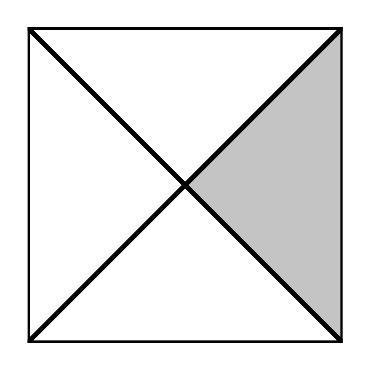
\begin{tikzpicture}[scale=2, line cap=round,line join=round,>=triangle 45,x=1.0cm,y=1.0cm]
\clip(0,0) rectangle (2,2);
\draw [line width=1.6pt] (0,0) -- (2,0) -- (1,1) -- cycle;
\fill [line width=1.6pt,fill=black,fill opacity=0.23] (2,0) -- (2,2) -- (1,1) -- cycle;
\draw [line width=1.6pt] (2,0) -- (2,2) -- (1,1) -- cycle;
\draw [line width=1.6pt] (1,1) -- (2,2) -- (0,2) -- cycle;
\draw [line width=1.6pt] (0,2) -- (0,0) -- (1,1) -- cycle;
\end{tikzpicture}}
    \item
\raisebox{-10em}{
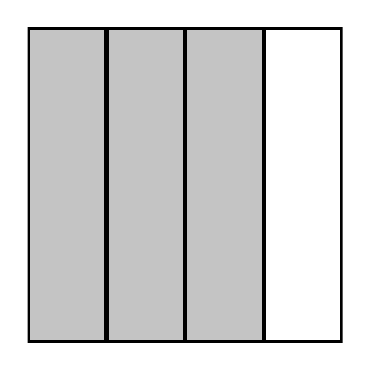
\begin{tikzpicture}[scale=2,line cap=round,line join=round,>=triangle 45,x=0.5cm,y=0.5cm]
\clip(0,0) rectangle (4,4);
\draw [line width=1.6pt] (0,0) -- (1,0) -- (1,4) -- (0,4) -- cycle;
\fill [line width=1.6pt,fill=black,fill opacity=0.23] (0,0) -- (1,0) -- (1,4) -- (0,4) -- cycle;
\draw [line width=1.6pt] (1,0) -- (2,0) -- (2,4) -- (1,4) -- cycle;
\fill [line width=1.6pt,fill=black,fill opacity=0.23] (1,0) -- (2,0) -- (2,4) -- (1,4) -- cycle;
\draw [line width=1.6pt] (2,0) -- (3,0) -- (3,4) -- (2,4) -- cycle;
\fill [line width=1.6pt,fill=black,fill opacity=0.23] (2,0) -- (3,0) -- (3,4) -- (2,4) -- cycle;
\draw [line width=1.6pt] (3,0) -- (4,0) -- (4,4) -- (3,4) -- cycle;
\end{tikzpicture}}
    \item
\raisebox{-10em}{
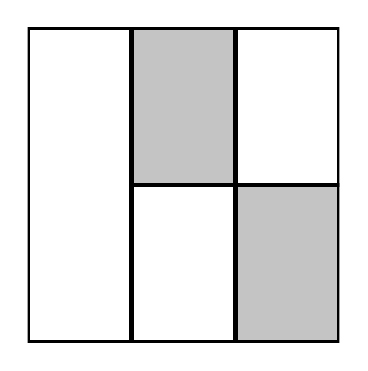
\begin{tikzpicture}[scale=2,line cap=round,line join=round,>=triangle 45,x=0.66cm,y=0.5cm]
\clip(0,0) rectangle (3,4);
\draw [line width=1.6pt] (0,0) -- (1,0) -- (1,4) -- (0,4) -- cycle;
\draw [line width=1.6pt] (1,0) -- (2,0) -- (2,2) -- (1,2) -- cycle;
\draw [line width=1.6pt] (1,2) -- (2,2) -- (2,4) -- (1,4) -- cycle;
\fill [line width=1.6pt,fill=black,fill opacity=0.23] (1,2) -- (2,2) -- (2,4) -- (1,4) -- cycle;
\draw [line width=1.6pt] (2,0) -- (3,0) -- (3,2) -- (2,2) -- cycle;
\draw [line width=1.6pt] (2,2) -- (3,2) -- (3,4) -- (2,4) -- cycle;
\fill [line width=1.6pt,fill=black,fill opacity=0.23] (2,0) -- (3,0) -- (3,2) -- (2,2) -- cycle;
\end{tikzpicture}}
  \end{enumerate}
\end{multicols}
\end{exercise}

\begin{solution}
\begin{multicols}{3}
\begin{enumerate}[(a)]
  \item $\dfrac{1}{4}$
  \item $\dfrac{3}{4}$
  \item $\dfrac{2}{6}$
\end{enumerate}
\end{multicols}
\end{solution}

\begin{exercise}
Een zak snoepjes wordt verdeeld onder 3 kinder. Evy krijgt 8 snoepjes, Tineke krijgt er 2 minder en Nele krijgt er 3. Druk uit door middel van een breuk hoeveel snoepjes uit de zak elk kind krijgt.
\end{exercise}

\begin{solution}
In de zak zitten $8 + 6 + 3 = 17$ snoepjes.
Het geheel bestaat uit $17$ delen; dus de noemer is $17$.
Evy krijgt $\dfrac{8}{17}$, Tineke $\dfrac{6}{17}$ en Nele $\dfrac{3}{17}$. 
\end{solution}

\subsection{Hoofdeigenschap van breuken}

We duiden van een rechthoek achtereenvolgens $\dfrac{2}{4}$, $\dfrac{1}{2}$ en $\dfrac{3}{6}$ aan.

\newcommand{\drawbox}[4]
{
\draw [line width=1.6pt] (#1,#2) -- (#3,#2) -- (#3,#4) -- (#1,#4) -- cycle;
}
\newcommand{\fillbox}[4]
{
\draw [line width=1.6pt] (#1,#2) -- (#3,#2) -- (#3,#4) -- (#1,#4) -- cycle;
\fill [fill opacity=0.23] (#1,#2) -- (#3,#2) -- (#3,#4) -- (#1,#4) -- cycle;
}

\begin{itemize}
  \item $\dfrac{2}{4}$\hspace*{1em}\raisebox{-1em}{
\begin{tikzpicture}[line cap=round,line join=round,>=triangle 45,x=1.0cm,y=1.0cm]
\clip(0,0) rectangle (6,1);
\fillbox{0}{0}{1.5}{1}
\fillbox{1.5}{0}{3}{1}
\drawbox{3}{0}{4.5}{1}
\drawbox{4.5}{0}{6}{1}
\end{tikzpicture}}
  \item $\dfrac{2}{4}$\hspace*{1em}\raisebox{-1em}{
\begin{tikzpicture}[line cap=round,line join=round,>=triangle 45,x=1.0cm,y=1.0cm]
\clip(0,0) rectangle (6,1);
\fillbox{0}{0}{3}{1}
\drawbox{3}{0}{6}{1}
\end{tikzpicture}}
  \item $\dfrac{3}{6}$\hspace*{1em}\raisebox{-1em}{
\begin{tikzpicture}[line cap=round,line join=round,>=triangle 45,x=1.0cm,y=1.0cm]
\clip(0,0) rectangle (6,1);
\fillbox{0}{0}{1}{1}
\fillbox{1}{0}{2}{1}
\fillbox{2}{0}{3}{1}
\drawbox{3}{0}{4}{1}
\drawbox{4}{0}{5}{1}
\drawbox{5}{0}{6}{1}
\end{tikzpicture}}
\end{itemize}

Het aangeduide deel is telkens even groot.
$$\dfrac{2}{4}=\dfrac{1}{2}=\dfrac{3}{6}$$

Dit kunnen we algebraïsch afleiden:
$$\dfrac{2}{4}=\dfrac{2:2}{4:2}=\dfrac{1}{2} \qquad\mbox{ en }\qquad\dfrac{1}{2}=\dfrac{1\cdot 3}{2\cdot 3}=\dfrac{3}{6}\;.$$

\begin{onthoud}
De waarde van een breuk verandert niet als we teller en noemer van die breuk vermenigvuldigen met of delen door eenzelfde van nul verschillend getal.
\end{onthoud}

\begin{exercise}
Vul de ontbrekende tellers en noemers in, zodat alle breuken gelijk zijn.
\begin{enumerate}[(a)]
  \item $\dfrac{3}{13}=\dfrac{\arule{0.75cm}}{78}=\dfrac{6}{\arule{0.75cm}}=\dfrac{90}{\arule{0.75cm}}$
  \item $\dfrac{27}{\arule{0.75cm}}=\dfrac{\arule{0.75cm}}{24}=\dfrac{9}{4}=\dfrac{45}{\arule{0.75cm}}$
\end{enumerate}
\end{exercise}

\begin{solution}
\begin{enumerate}[(a)]
  \item $\dfrac{3}{13}=\dfrac{18}{78}=\dfrac{6}{26}=\dfrac{90}{390}$
  \item $\dfrac{27}{12}=\dfrac{54}{24}=\dfrac{9}{4}=\dfrac{45}{20}$
\end{enumerate}
\end{solution}

\begin{exercise}
Bepaal telkens de waarde van $a$.
\begin{enumerate}[(a)]
  \item $\dfrac{25}{55}=\dfrac{5}{a}$
  \item $\dfrac{a}{12}=\dfrac{13}{6}$
\end{enumerate}
\end{exercise}

\begin{solution}
\begin{enumerate}[(a)]
  \item $a=55:5=11$
  \item $a=13\cdot 2=26$
\end{enumerate}
\end{solution}

\subsection{Vereenvoudigen van breuken}

Om een breuk te vereenvoudigen, deel je teller en noemer door eenzelfde getal.
Een breuk waarvan teller en noemer geen gemeenschappelijke deler hebben, is een {\em onvereenvoudigbare breuk}. 

Als we bewerkingen uitvoeren met breuken, herleiden we de breuken altijd tot hun eenvoudigste vorm.
Hiervoor bepalen we de g.g.d. van teller en noemer.

\begin{voorbeeld}
Herleid tot een onvereenvoudigbare breuk:
$$\dfrac{24}{102}=\dfrac{?}{?}$$

We ontbinden teller en noemer in factoren:
\begin{center}
\begin{tabular}{r|lp{2cm}r|l}
24 & 2 & & 102 & 2\\
12 & 2 & &  52 & 3\\
6 & 2  & &  17 & 17\\
3 & 3  & &   1\\
1
\end{tabular}
\end{center}
Ontbonden in factoren hebben we dus $24=2^3\cdot 3$ en $102=2\cdot 3 \cdot 17$\\

Nu bepalen we de grootste gemene deler: $ggd(24,102)=2\cdot 3=6$.\\

En dus $\dfrac{24}{102}=\dfrac{24:6}{102:6}=\dfrac{4}{17}$.

\end{voorbeeld}

Een andere manier om een breuk te herleiden tot een onvereenvoudigbare breuk is:
\begin{itemize}
  \item ontbind teller en noemer in priemfactoren;
  \item schrap de gemeenschappelijke factoren.
\end{itemize}

\begin{voorbeeld}
$$\dfrac{24}{102}=\dfrac{2\cdot 2\cdot 2\cdot 3}{2\cdot 3 \cdot 17}=\dfrac{\cancel{2}\cdot 2\cdot 2\cdot \cancel{3}}{\cancel{2}\cdot \cancel{3} \cdot 17}=\dfrac{4}{17}$$
\end{voorbeeld}

\begin{voorbeeld}
$$\dfrac{275}{495}=\dfrac{?}{?}$$

\begin{center}
\begin{tabular}{r|lp{2cm}r|l}
275 & 5 & & 495 & 3\\
55 & 5 & &  165 & 3\\
11 & 11  & &  55 & 5\\
1 &   & &   11 & 11\\
  &   & &    1 &\\
\multicolumn{2}{c}{$275=5^2\cdot 11$}&&\multicolumn{2}{c}{$495=3^2\cdot 5\cdot 11$}
\end{tabular}
\end{center}

\paragraph*{Eerste manier:}
$$\ggd(275, 495)=5  \cdot 11 = 55$$
$$\Rightarrow \dfrac{275}{495}=\dfrac{275:55}{495:55}=\dfrac{5}{9}$$

\paragraph*{Tweede manier:}
$$\dfrac{275}{495}=\dfrac{\cancel{5}\cdot 5\cdot \cancel{11}}{3 \cdot 3 \cdot \cancel{5} \cdot \cancel{11}}=\dfrac{5}{9}$$

\end{voorbeeld}

\begin{exercise}
Herleid tot een onvereenvoudigbare breuk:
\begin{enumerate}[(a)]
  \item uit het hoofd:
  %\begin{multicols}{2}
  \begin{itemize}
    \item $\dfrac{6}{15}$
    \item $\dfrac{22}{55}$
  \end{itemize}
  %\end{multicols}
  \item door middel van de $\ggd$:
  %\begin{multicols}{2}
  \begin{itemize}
    \item $\dfrac{540}{756}$
    \item $\dfrac{1089}{1078}$
  \end{itemize}
  %\end{multicols}
  \item door teller en noemer te ontbinden in priemfactoren en dan te vereenvoudigen:
  %\begin{multicols}{2}
  \begin{itemize}
    \item $\dfrac{658}{1128}$
    \item $\dfrac{11067}{15470}$
  \end{itemize}
  %\end{multicols}
\end{enumerate}
\end{exercise}

\begin{solution}
\begin{enumerate}[(a)]
  \item \begin{itemize}
    \item $\dfrac{6}{15}=\dfrac{2}{5}$
    \item $\dfrac{22}{55}=\dfrac{2}{5}$
  \end{itemize}
  \item \begin{itemize}
    \item
    \begin{tabular}[t]{r|lp{2cm}r|l}
    540 & 2  & &  756 & 2\\
    270 & 2  & &  378 & 2\\
    135 & 3  & &  189 & 3\\
     45 & 3  & &   63 & 3\\
     15 & 3  & &   21 & 3\\
      5 & 5  & &    7 & 7\\
      1 &    & &    1 &  \\
    \multicolumn{2}{c}{$540=2^2\cdot 3^3\cdot 5$}
    &&\multicolumn{2}{c}{$756=2^2\cdot 3^3 \cdot 7$}
    \end{tabular}
    
    $\Rightarrow \ggd(540,756)=2^2\cdot 3^3 = 4\cdot 27= 108$\\[1em]
    $\Rightarrow \dfrac{540}{756}=\dfrac{540:108}{756:108}=\dfrac{5}{7}$
    \item
    \begin{tabular}[t]{r|lp{2cm}r|l}
    1089 & 3  & & 1078 & 2  \\
     363 & 3  & &  539 & 7  \\
     121 & 11 & &   77 & 7  \\
      11 & 11 & &   11 & 11 \\
       1 &    & &    1 &    \\
    \multicolumn{2}{c}{$1089=3^2\cdot 11^2$}
    &&\multicolumn{2}{c}{$1078=2\cdot 7^2\cdot 11$}
    \end{tabular}
    
    $\Rightarrow \ggd(1089,1078)=11$\\[1em]
    $\Rightarrow \dfrac{1089}{1078}=\dfrac{99}{98}$
  \end{itemize}
  \item \begin{itemize}
    \item
    \begin{tabular}[t]{r|lp{2cm}r|l}
    658 & 2  & & 1128 &  2\\
    329 & 7  & &  564 &  2\\
     47 & 47 & &  282 &  2\\
      1 &    & &  141 &  3\\
    \multicolumn{2}{c}{$658=2\cdot 7\cdot 47$}& &   47 & 47\\
    \multicolumn{2}{c}{}& &    1 &   \\
    \multicolumn{2}{c}{}
    &&\multicolumn{2}{c}{$1128=2^3\cdot 3\cdot 47$}
    \end{tabular}
    
    $\Rightarrow \dfrac{658}{1128}=\dfrac{\cancel{2}\cdot 7\cdot \cancel{47}}{2\cdot \cancel{2}\cdot 2\cdot 3\cdot \cancel{47}}=\dfrac{7}{12}$\\
    \item
    \begin{tabular}[t]{r|lp{2cm}r|l}
    11067 & 3  & & 15470 &  2\\
     3689 & 7  & &  7735 &  5\\
      527 & 17 & &  1547 &  7\\
       31 & 31 & &   221 & 13\\
        1 &    & &    17 & 17\\
    \multicolumn{2}{c}{$11067=3\cdot7\cdot17\cdot31$}& &   1 & \\
    \multicolumn{2}{c}{}
    &&\multicolumn{2}{c}{$15470=\cdot2\cdot5\cdot7\cdot13\cdot17$}
    \end{tabular}
    
    $\Rightarrow \dfrac{11067}{15470}=\dfrac{3\cdot\cancel{7}\cdot \cancel{17}\cdot 31}{2\cdot 5\cdot \cancel{7}\cdot 13\cdot \cancel{17}}=\dfrac{93}{130}$\\
    
    \end{itemize}
\end{enumerate}
\end{solution}

\subsection{Gelijknamig maken van breuken}

Breuken met dezelfde noemer, noemt men gelijknamige breuken.
Breuken gelijknamig maken betekent beide breuken herleiden naar een breuk met dezelfde noemer.
We nemen deze gemeenschappelijke noemer steeds zo klein mogelijk.
We zoeken dus telkens het kleinste gemeen veelvoud van de gegeven noemers.


\begin{voorbeeld}
Maak $\dfrac{5}{6}$ en $\dfrac{3}{4}$ gelijknamig

$\kgv(6,4)=12$\\

$\dfrac{5}{6}= \dfrac{5\times 2}{6\times 2}=\dfrac{10}{12}$

We vermenigvuldigen de noemer met $2$. Om een gelijkwaardige breuk te bekomen, vermenigvuldigen we ook de teller met $2$. (hoofdeigenschap van breuken)\\

$\dfrac{3}{4}= \dfrac{3\times 3}{4\times 3}=\dfrac{9}{12}$ \qquad Teller en noemer $\times 3$.\\

De gelijknamige breuken zijn $\dfrac{10}{12}$ en $\dfrac{9}{12}$.
\end{voorbeeld}

\begin{voorbeeld}
Maak gelijknamig: $\dfrac{3}{8}$ en $\dfrac{5}{9}$

$\kgv(8,9)=72$\\

$\dfrac{3}{8}= \dfrac{3\times 9}{8\times 9}=\dfrac{27}{72}$ en
$\dfrac{5}{9}= \dfrac{5\times 8}{9\times 8}=\dfrac{40}{72}$

De gelijknamige breuken zijn $\dfrac{27}{72}$ en $\dfrac{40}{72}$.
\end{voorbeeld}

\begin{voorbeeld}
Maak gelijknamig: $\dfrac{12}{45}$ en $\dfrac{21}{75}$

Controleer eerst of je de gegeven breuk kan vereenvoudigen en maak daarna gelijknamig.

\begin{itemize}
  \item vereenvoudig\\
  $\dfrac{12}{45}=\dfrac{4}{15}$ en $\dfrac{21}{75}=\dfrac{7}{25}$
  \item maak gelijknamig\\
  $\kgv(15,25)=75$\\
  $\dfrac{4}{15}= \dfrac{20}{75}$ en
  $\dfrac{7}{25}= \dfrac{21}{75}$
\end{itemize}
\end{voorbeeld}

\begin{exercise}
Maak volgende breuken gelijknamig:
\begin{enumerate}[(a)]
  \item $\dfrac{5}{6}$ en $\dfrac{3}{8}$
  \item $\dfrac{60}{96}$ en $\dfrac{45}{66}$
  \item $\dfrac{4}{6}$ en $\dfrac{6}{8}$ en $\dfrac{3}{9}$
\end{enumerate}
\end{exercise}

\begin{solution}
\begin{enumerate}[(a)]
  \item $\dfrac{5}{6}=\dfrac{20}{24}$ en $\dfrac{5}{6}=\dfrac{20}{24}$
  \item vereenvoudig: $\dfrac{60}{96}=\dfrac{5}{8}$ en $\dfrac{45}{66}=\dfrac{15}{22}$\\
  gemeenschappelijke noemer: $88$\\
  gelijknamig maken: $\dfrac{5}{8}=\dfrac{55}{88}$ en $\dfrac{15}{22}=\dfrac{60}{88}$
  \item vereenvoudig: $\dfrac{2}{3}$ en $\dfrac{3}{4}$ en $\dfrac{1}{3}$\\
  gemeenschappelijke noemer: $12$\\
  gelijknamig maken: $\dfrac{8}{12}$ en $\dfrac{9}{12}$ en $\dfrac{4}{12}$\\
\end{enumerate}
\end{solution}

\subsection{Ordenen van breuken}

d.w.z. rangschikken van breuken van klein naar groot of van groot naar klein.

\subsubsection{Gelijknamige breuken}

De breuk met de kleinste teller is de kleinste breuk.
$$\dfrac{2}{7} < \dfrac{5}{7}$$

\subsubsection{Breuken met gelijke teller}

Bij breuken met gelijke teller is de breuk met de grootste noemer het kleinst

\begin{itemize}
  \item $\dfrac{2}{6}$\hspace*{1em}\raisebox{-1em}{
\begin{tikzpicture}[line cap=round,line join=round,>=triangle 45,x=1.0cm,y=1.0cm]
\clip(0,0) rectangle (6,1);
\fillbox{0}{0}{1}{1}
\fillbox{1}{0}{2}{1}
\drawbox{2}{0}{3}{1}
\drawbox{3}{0}{4}{1}
\drawbox{4}{0}{5}{1}
\drawbox{5}{0}{6}{1}
\end{tikzpicture}}
  \item $\dfrac{2}{4}$\hspace*{1em}\raisebox{-1em}{
\begin{tikzpicture}[line cap=round,line join=round,>=triangle 45,x=1.0cm,y=1.0cm]
\clip(0,0) rectangle (6,1);
\fillbox{0}{0}{1.5}{1}
\fillbox{1.5}{0}{3}{1}
\drawbox{3}{0}{4.5}{1}
\drawbox{4.5}{0}{6}{1}
\end{tikzpicture}}
\end{itemize}

$$\dfrac{2}{6} < \dfrac{2}{4}$$

\subsubsection{Ongelijknamige breuken}

\begin{voorbeeld}
Welke breuk is het grootst?
$$\dfrac{7}{9} \mbox{ of } \dfrac{11}{15}$$
Maak de breuken eerst gelijknamig en vergelijk ze dan:\\
$\dfrac{7}{9}=\dfrac{35}{45}$ en $\dfrac{11}{15}=\dfrac{33}{45}$\\
$\dfrac{35}{45}>\dfrac{33}{45}$ dus:
$$\dfrac{7}{9}>\dfrac{11}{15}$$
\end{voorbeeld}

\begin{exercise}
Rangschik van klein naar groot:
$$\dfrac{12}{30} \qquad \dfrac{21}{28} \qquad \dfrac{36}{18} \qquad \dfrac{3}{5}$$
\end{exercise}

\begin{solution}
$$\dfrac{12}{30} \qquad \dfrac{21}{28} \qquad \dfrac{36}{18} \qquad \dfrac{3}{5}$$
Vereenvoudigen:
$$\dfrac{2}{5} \qquad \dfrac{3}{4} \qquad \dfrac{2}{1} \qquad \dfrac{3}{5}$$
Gelijknamig maken:
$$\dfrac{8}{20} \qquad \dfrac{15}{20} \qquad \dfrac{40}{20} \qquad \dfrac{12}{20}$$
Ordenen:
$$\dfrac{8}{20}  < \dfrac{12}{20} < \dfrac{15}{20} < \dfrac{40}{20}$$
Dus:
$$\dfrac{12}{30}  < \dfrac{3}{5} < \dfrac{21}{28} < \dfrac{36}{18}$$
\end{solution}

\begin{exercise}
Plaats het ongelijkheidsteken $<$ of $>$
\begin{multicols}{2}
\begin{enumerate}[(a)]
  \item $\dfrac{1}{7} \quad\arule{1cm}\quad \dfrac{1}{8}$
  \item $\dfrac{35}{41} \quad\arule{1cm}\quad \dfrac{31}{41}$
  \item $\dfrac{5}{12} \quad\arule{1cm}\quad \dfrac{5}{9}$
  \item $\dfrac{7}{20} \quad\arule{1cm}\quad \dfrac{9}{25}$
  \item $\dfrac{3}{14} \quad\arule{1cm}\quad \dfrac{4}{21}$
  \item $\dfrac{5}{9} \quad\arule{1cm}\quad \dfrac{5}{7}$
\end{enumerate}
\end{multicols}
\end{exercise}

\begin{solution}
\begin{multicols}{2}
\begin{enumerate}[(a)]
  \item $\dfrac{1}{7} > \dfrac{1}{8}$
  \item $\dfrac{35}{41} > \dfrac{31}{41}$
  \item $\dfrac{5}{12} < \dfrac{5}{9}$
  \item $\dfrac{7}{20} < \dfrac{9}{25}$
  \item $\dfrac{3}{14} > \dfrac{4}{21}$
  \item $\dfrac{5}{9} < \dfrac{5}{7}$
\end{enumerate}
\end{multicols}
\end{solution}

\begin{onthoud}
\begin{itemize}
  \item Hoofdeigenschap van breuken:\\
  De waarde van een breuk verandert niet als je teller en noemer vermenigvuldigt met, of deelt door eenzelfde van nul verschillend getal.
  \item Breuken vereenvoudigen:\\
  Deel teller en noemer door hun grootste gemene deler.
  \item Breuken gelijknamig maken:
  \begin{itemize}
    \item Vereenvoudig, indien mogelijk, de gegeven breuken.
    \item De gemeenschappelijke noemer is het k.g.v. van beide noemers.
  \end{itemize}
  \item Ordenen van breuken:
  \begin{itemize}
    \item Vereenvoudig eerst de gegeven breuken.
    \item Maak de breuken gelijknamig.
    \item Rangschik de gelijknamige breuken.
    \item Noteer de breuken in hun oorspronkelijke vorm, in de juiste volgorde.
  \end{itemize}
\end{itemize}
\end{onthoud}

\newpage
\section*{Oplossingen A.C.O.}

\immediate\closeout\solutionstream
\input{\jobname.sol}

\end{document}


\begin{voorbeeld}
\end{voorbeeld}

\begin{exercise}
\end{exercise}

\begin{solution}
\end{solution}
